\documentclass{Supervised_Reinforcement_Learningqsport}
\usepackage{amsmath,amssymb,float}
\usepackage{graphicx}
\usepackage{booktabs}
\usepackage{float}
\usepackage{array}

\begin{document}

\title{Análise do Impacto da Exploração na Aprendizagem Off-Policy}

\author{Luan Ornelas de Souza, Daniel E. Higa
\thanks{Luan Ornelas de Souza e Daniel E. Higa¸
Faculdade de Engenharia Elétrica e de Computação (FEEC), Universidade Estadual de Campinas (UNICAMP), Campinas-SP. E-mails: d992741@dac.unicamp.br,
l299739@dac.unicamp.br .}}

\maketitle

\markboth{IA368FF - INTRODUÇÃO AO APRENDIZADO POR REFORÇO - 2026-1º SEMESTRE} {IA368FF - INTRODUÇÃO AO APRENDIZADO POR REFORÇO - 2026-1º SEMESTRE}

\begin{resumo}
Este trabalho investiga como diferentes níveis de exploração afetam o desempenho de dois algoritmos off-policy amplamente utilizados em Deep Reinforcement Learning: Soft Actor-Critic (SAC) e Twin Delayed Deep Deterministic Policy Gradient (TD3).

\end{resumo}

\section{Descrição do Problema}

SAC e TD3 adotam filosofias distintas: o SAC incorpora a exploração diretamente na função objetivo por meio da maximização da entropia, enquanto o TD3 promove exploração por meio da adição de ruído às ações.

\subsection{Soft Actor-Critic (SAC)}

O SAC (Haarnoja et al., 2018) é um algoritmo \textit{off-policy} baseado no princípio de \textbf{máxima entropia}. Sua função objetivo estendida é:

\begin{equation}
J(\pi) = \sum_{t=0}^{T} \mathbb{E}_{(s_t,a_t)\sim\rho_{\pi}}
\left[
r(s_t,a_t) + \alpha \, \mathcal{H}\bigl(\pi(\cdot|s_t)\bigr)
\right]
\end{equation}

onde $\alpha$ é o coeficiente de temperatura que balanceia recompensa e entropia. Um valor maior de $\alpha$ induz maior exploração, enquanto valores menores favorecem a explotação.

\textbf{Características:}
\begin{itemize}
    \item Política estocástica naturalmente exploradora;
    \item Duplo crítico para reduzir \textit{overestimation};
    \item $\alpha$ pode ser ajustado automaticamente.
\end{itemize}

\subsection{Twin Delayed Deep Deterministic Policy Gradient (TD3)}

O TD3 (Fujimoto et al., 2018) melhora o DDPG introduzindo:

\begin{itemize}
    \item \textbf{Twin Critics}: dois Q-networks para reduzir \textit{overestimation};
    \item \textbf{Delayed Policy Updates}: ator atualizado com menor frequência;
    \item \textbf{Target Policy Smoothing}: ruído adicionado às ações da política-alvo.
\end{itemize}

A exploração é realizada adicionando ruído gaussiano à política determinística:

\begin{equation}
a_t = \mu_{\theta}(s_t) + \epsilon,
\qquad
\epsilon \sim \mathcal{N}(0,\sigma^2)
\end{equation}

\subsection{Comparação dos Mecanismos de Exploração}

\begin{table}[H]
\centering
\caption{Comparação entre os mecanismos de exploração do SAC e TD3.}
\label{tab:sac_td3_comparison}
\begin{tabular}{|l|c|c|}
\hline
\textbf{Aspecto} & \textbf{SAC} & \textbf{TD3} \\
\hline
Tipo de política & Estocástica & Determinística + ruído \\
\hline
Exploração & Intrínseca (via entropia) & Extrínseca (perturbação) \\
\hline
Parâmetro & $\alpha$ (temperatura) & $\sigma$ (desvio-padrão do ruído) \\
\hline
\end{tabular}
\end{table}


\section{Métodos e Implementação}
Foram realizados um total de 130 experimentos no ambiente \texttt{Pendulum-v1} da biblioteca \textit{Gymnasium}, considerando diferentes configurações dos algoritmos Soft Actor-Critic (SAC) e Twin Delayed Deep Deterministic Policy Gradient (TD3). Para o algoritmo SAC, foram avaliados sete valores do coeficiente de entropia, $\alpha \in \{0.01, 0.05, 0.10, 0.20, \text{auto}, 0.40, 0.60\}$. Para o algoritmo TD3, foram considerados seis valores para o desvio-padrão do ruído de exploração, $\sigma \in \{0.05, 0.10, 0.20, 0.30, 0.50, 0.70\}$. Cada configuração foi treinada utilizando 10 diferentes sementes (\textit{seeds}), numeradas de 1 a 10, durante um total de 100\,000 passos de interação com o ambiente. Após o treinamento, cada política foi avaliada de forma determinística por meio da execução de 20 episódios, sendo utilizada a média das recompensas obtidas como medida de desempenho.

\subsection{Configuração Experimental}

O ambiente utilizado nos experimentos foi o \texttt{Pendulum-v1}, disponível na biblioteca \textit{Gymnasium}. O vetor de estado é composto por
$\left[\cos(\theta), \sin(\theta), \dot{\theta}\right] \in \mathbb{R}^{3}$,
enquanto a ação corresponde a um torque contínuo limitado ao intervalo
$[-2,2]$. A função de recompensa é dada por

\[
r = -\left(\theta^{2} + 0.1\,\dot{\theta}^{2} + 0.001\,u^{2}\right),
\]

cujo valor máximo é aproximadamente igual a zero, sendo alcançado quando o pêndulo permanece na posição vertical com velocidade angular nula e mínimo esforço de controle.

Os hiperparâmetros comuns utilizados em todas as configurações experimentais são apresentados na Tabela~\ref{tab:hiperparametros}.

\begin{table}[ht]
\centering
\caption{Hiperparâmetros comuns utilizados nos experimentos.}
\label{tab:hiperparametros}
\begin{tabular}{lc}
\hline
\textbf{Parâmetro} & \textbf{Valor} \\
\hline
Learning rate & $3 \times 10^{-4}$ \\
Buffer size & 100\,000 \\
Batch size & 256 \\
$\tau$ (soft update) & 0.005 \\
$\gamma$ (fator de desconto) & 0.99 \\
Learning starts & 1\,000 \\
Total timesteps & 100\,000 \\
Seeds & 1--10 \\
Episódios de avaliação & 20 \\
\hline
\end{tabular}
\end{table}

As configurações de exploração avaliadas para os algoritmos SAC e TD3 são apresentadas na Tabela~\ref{tab:exploracao}.

\begin{table}[H]
\centering
\caption{Configurações de exploração utilizadas para os algoritmos SAC e TD3.}
\label{tab:exploracao}
\begin{tabular}{ccc}
\hline
\textbf{Algoritmo} & \textbf{Configuração} & \textbf{Parâmetro} \\
\hline
SAC & SAC-1 & $\alpha = 0.01$ \\
SAC & SAC-2 & $\alpha = 0.05$ \\
SAC & SAC-3 & $\alpha = 0.10$ \\
SAC & SAC-4 & $\alpha = 0.20$ \\
SAC & SAC-5 & $\alpha = \text{auto}$ \\
SAC & SAC-6 & $\alpha = 0.40$ \\
SAC & SAC-7 & $\alpha = 0.60$ \\
TD3 & TD3-1 & $\sigma = 0.05$ \\
TD3 & TD3-2 & $\sigma = 0.10$ \\
TD3 & TD3-3 & $\sigma = 0.20$ \\
TD3 & TD3-4 & $\sigma = 0.30$ \\
TD3 & TD3-5 & $\sigma = 0.50$ \\
TD3 & TD3-6 & $\sigma = 0.70$ \\
\hline
\end{tabular}
\end{table}

\section{Resultados}

\subsection{Curvas de Aprendizado}

As curvas abaixo mostram a evolução da recompensa por episódio utilizando uma média móvel com janela de 20 episódios e intervalo de confiança de 95\% entre as diferentes \textit{seeds}.

\begin{figure}[H]
    \centering
    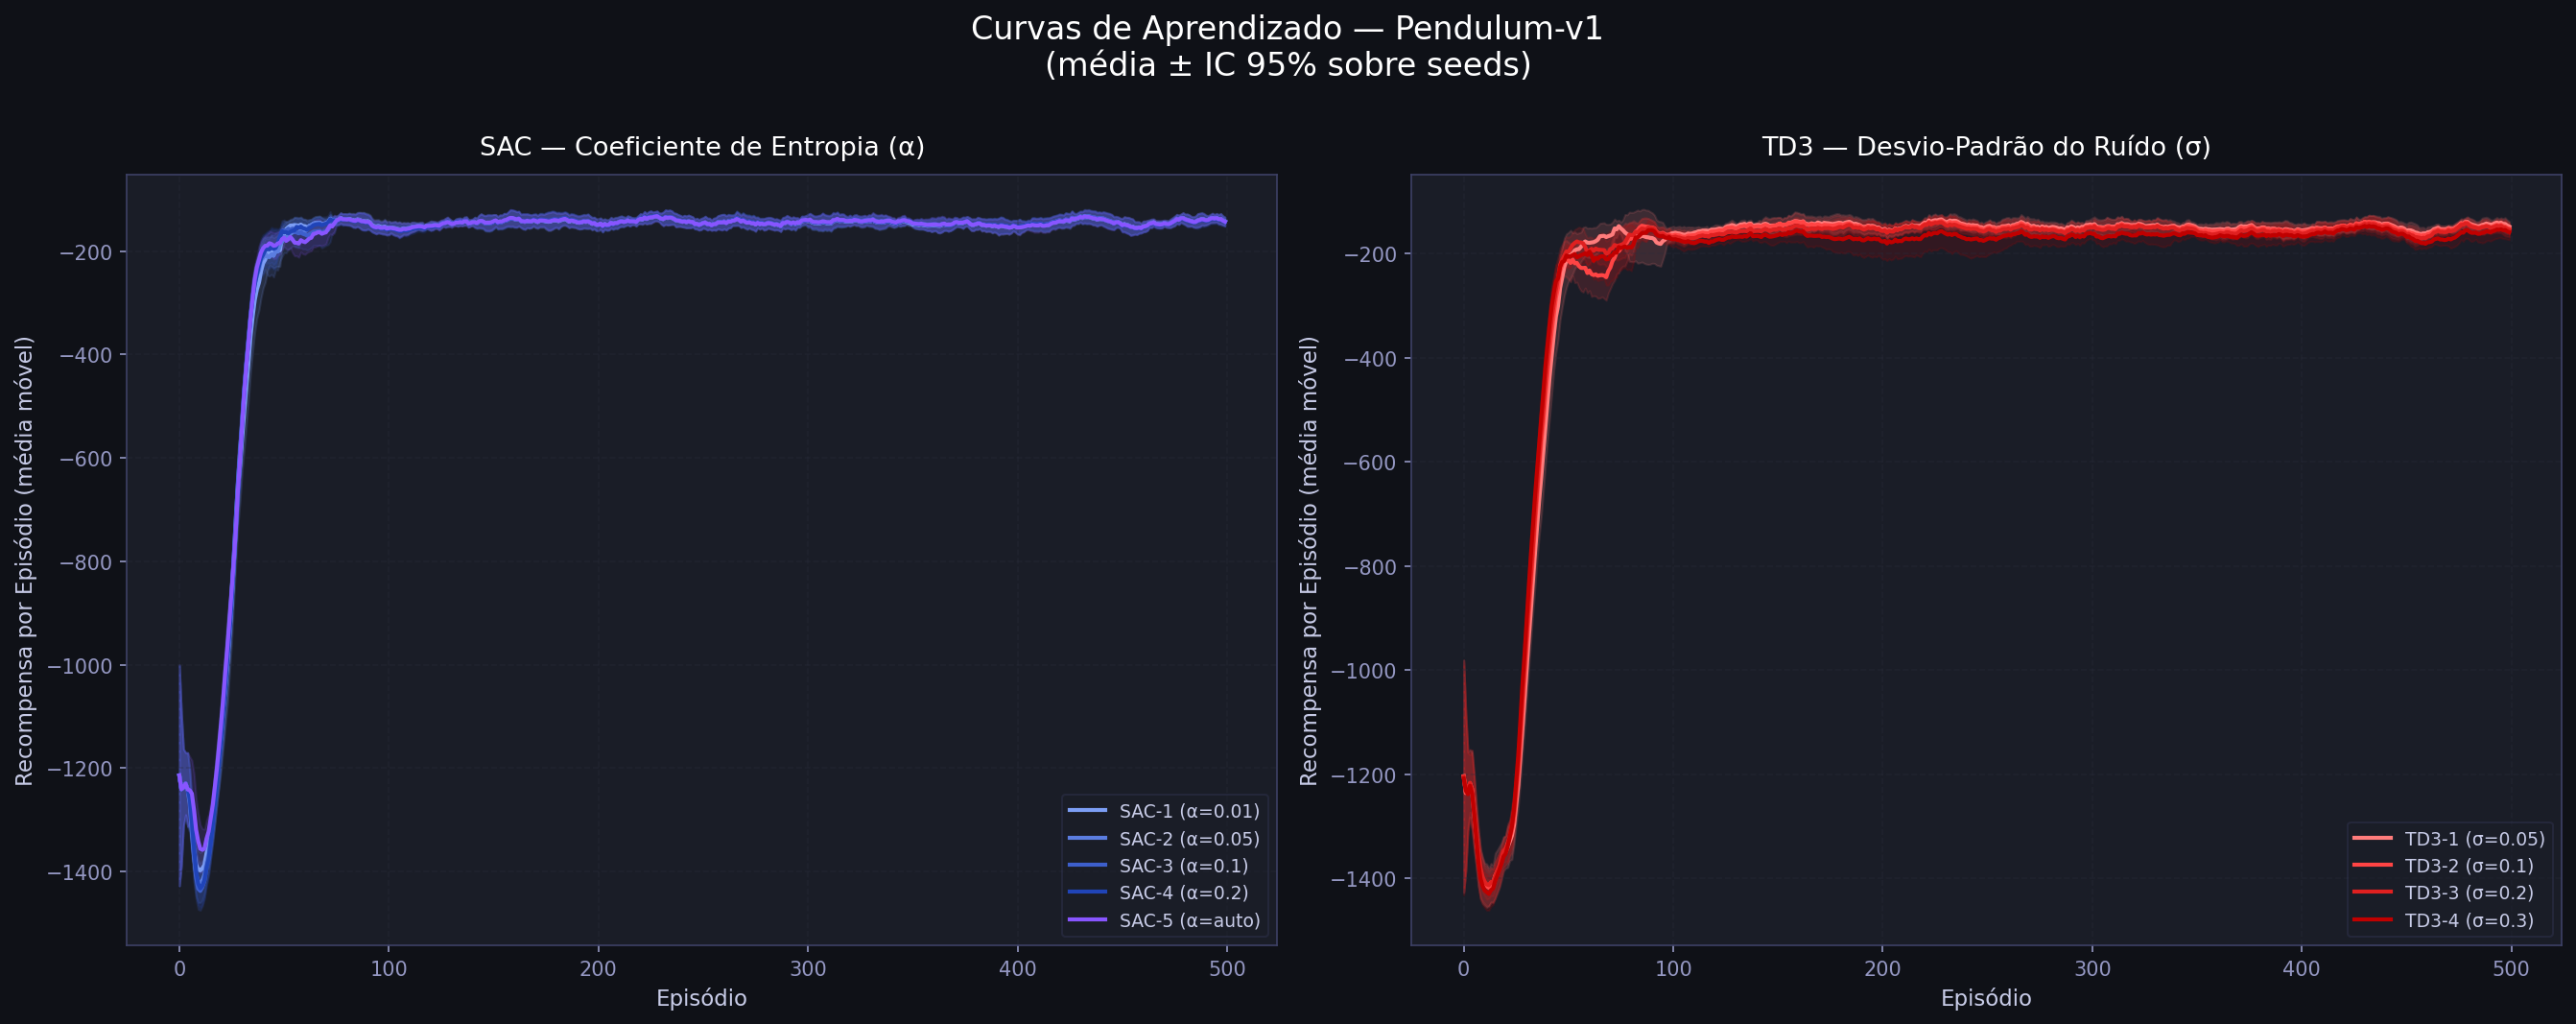
\includegraphics[width=0.95\columnwidth]{project/figures/learning_curves}
    
    \caption{Curvas de aprendizado dos algoritmos avaliados.}
    \label{fig:learning_curves}
\end{figure}

\textbf{Observações:}
\begin{itemize}
    \item O SAC tende a apresentar convergência mais suave e estável devido à exploração intrínseca baseada em entropia.
    \item O TD3 pode apresentar maior variância entre \textit{seeds}, dependendo do valor de $\sigma$ utilizado.
    \item Configurações com exploração insuficiente ou excessiva apresentam convergência mais lenta.
\end{itemize}

\subsection{Distribuição da Recompensa Final}

\begin{figure}[H]
    \centering
    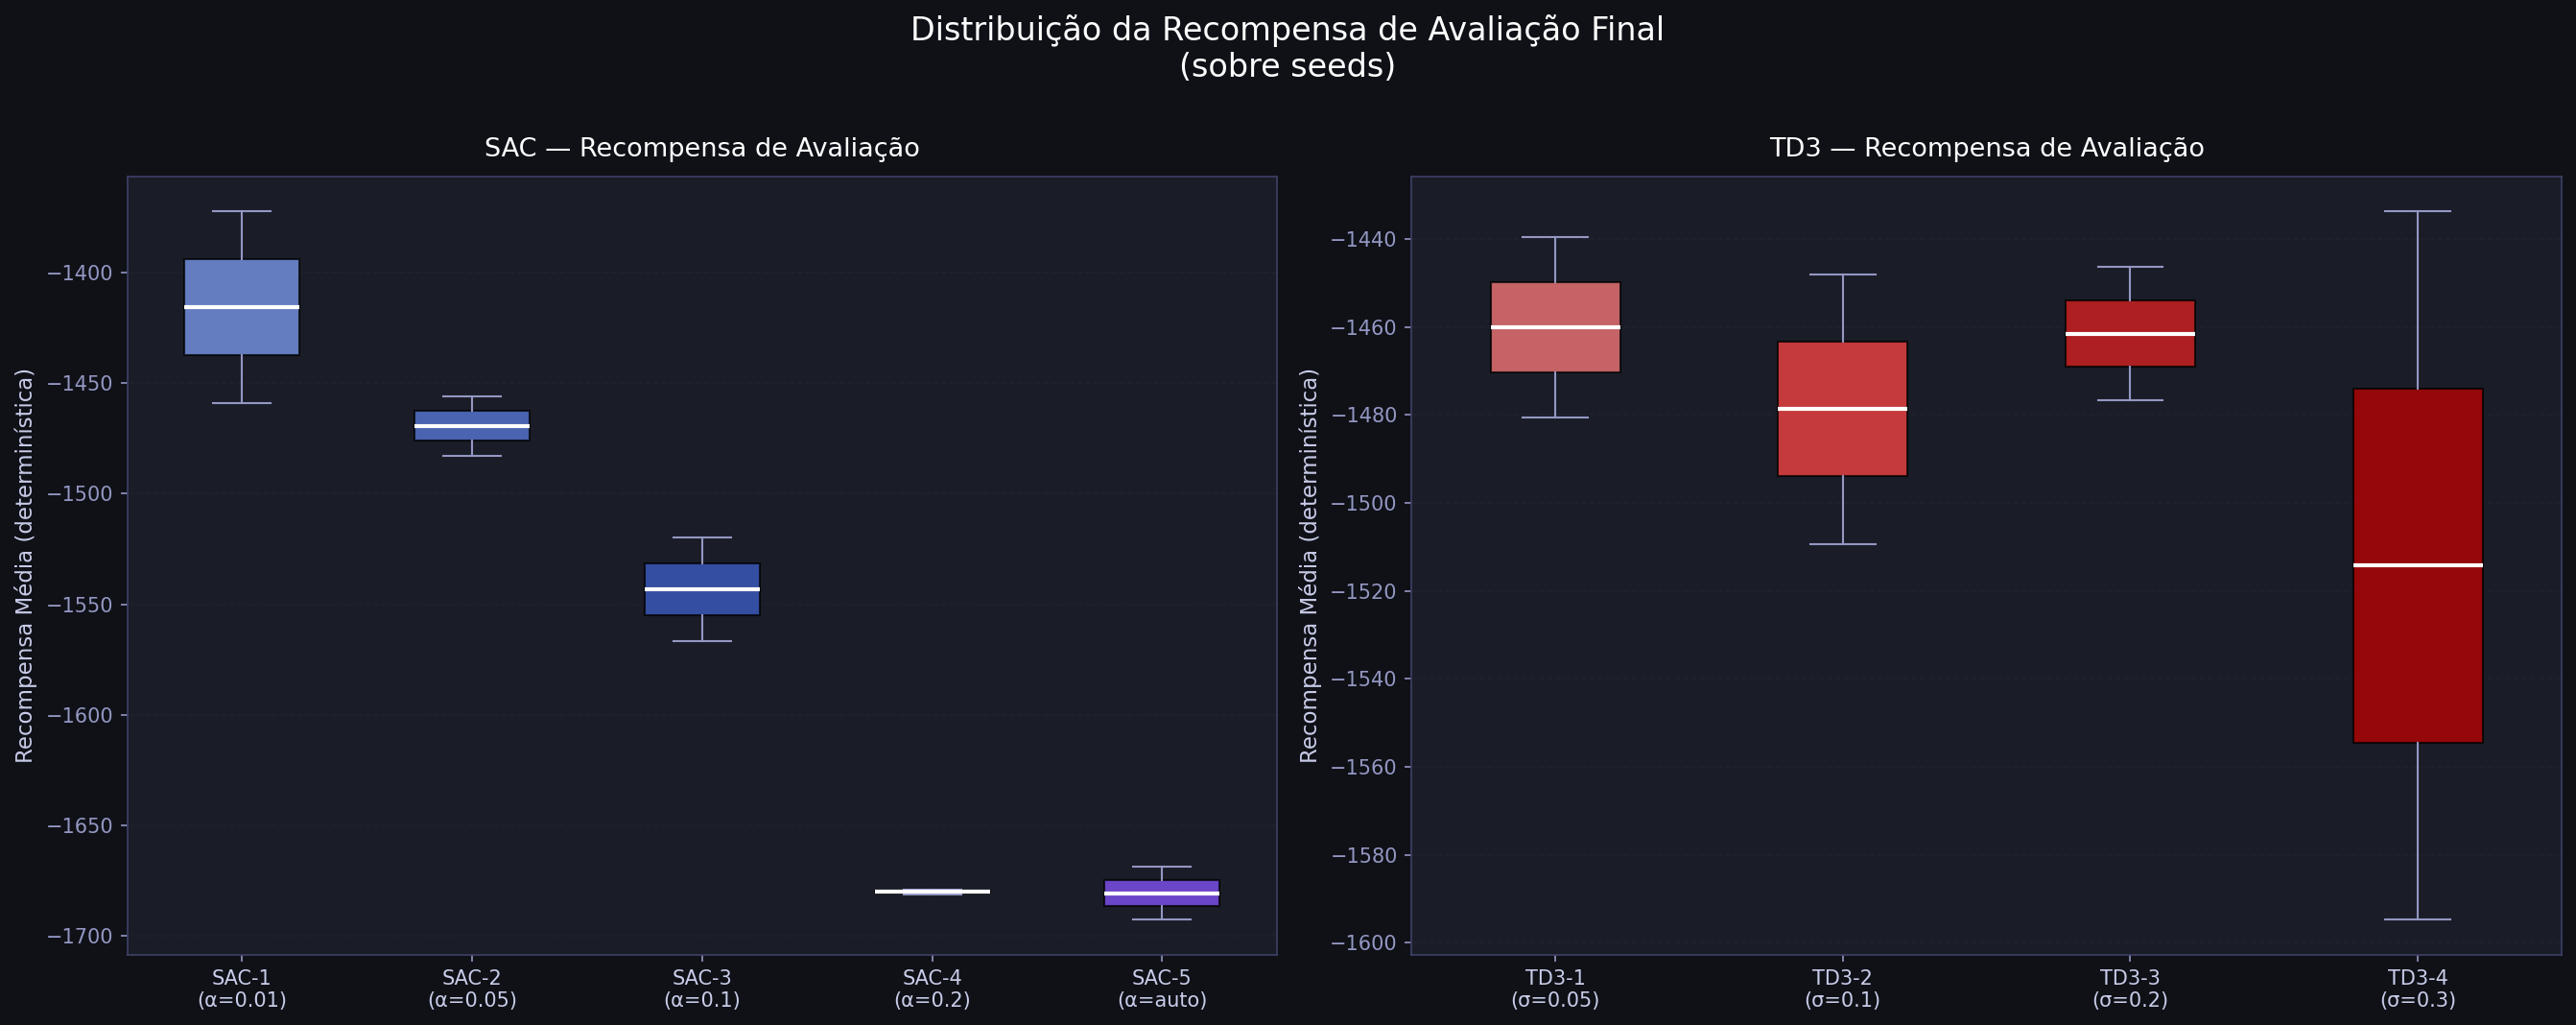
\includegraphics[width=0.95\columnwidth]{project/figures/boxplots_final_reward}
    \caption{Boxplots da recompensa final obtida por cada configuração.}
    \label{fig:boxplots_final_reward}
\end{figure}

A largura das caixas indica a variabilidade entre as diferentes \textit{seeds}. A configuração SAC-5 ($\alpha=\mathrm{auto}$) tende a apresentar um bom equilíbrio entre desempenho e estabilidade.

\subsection{Impacto do Parâmetro de Exploração}

\begin{figure}[H]
    \centering
    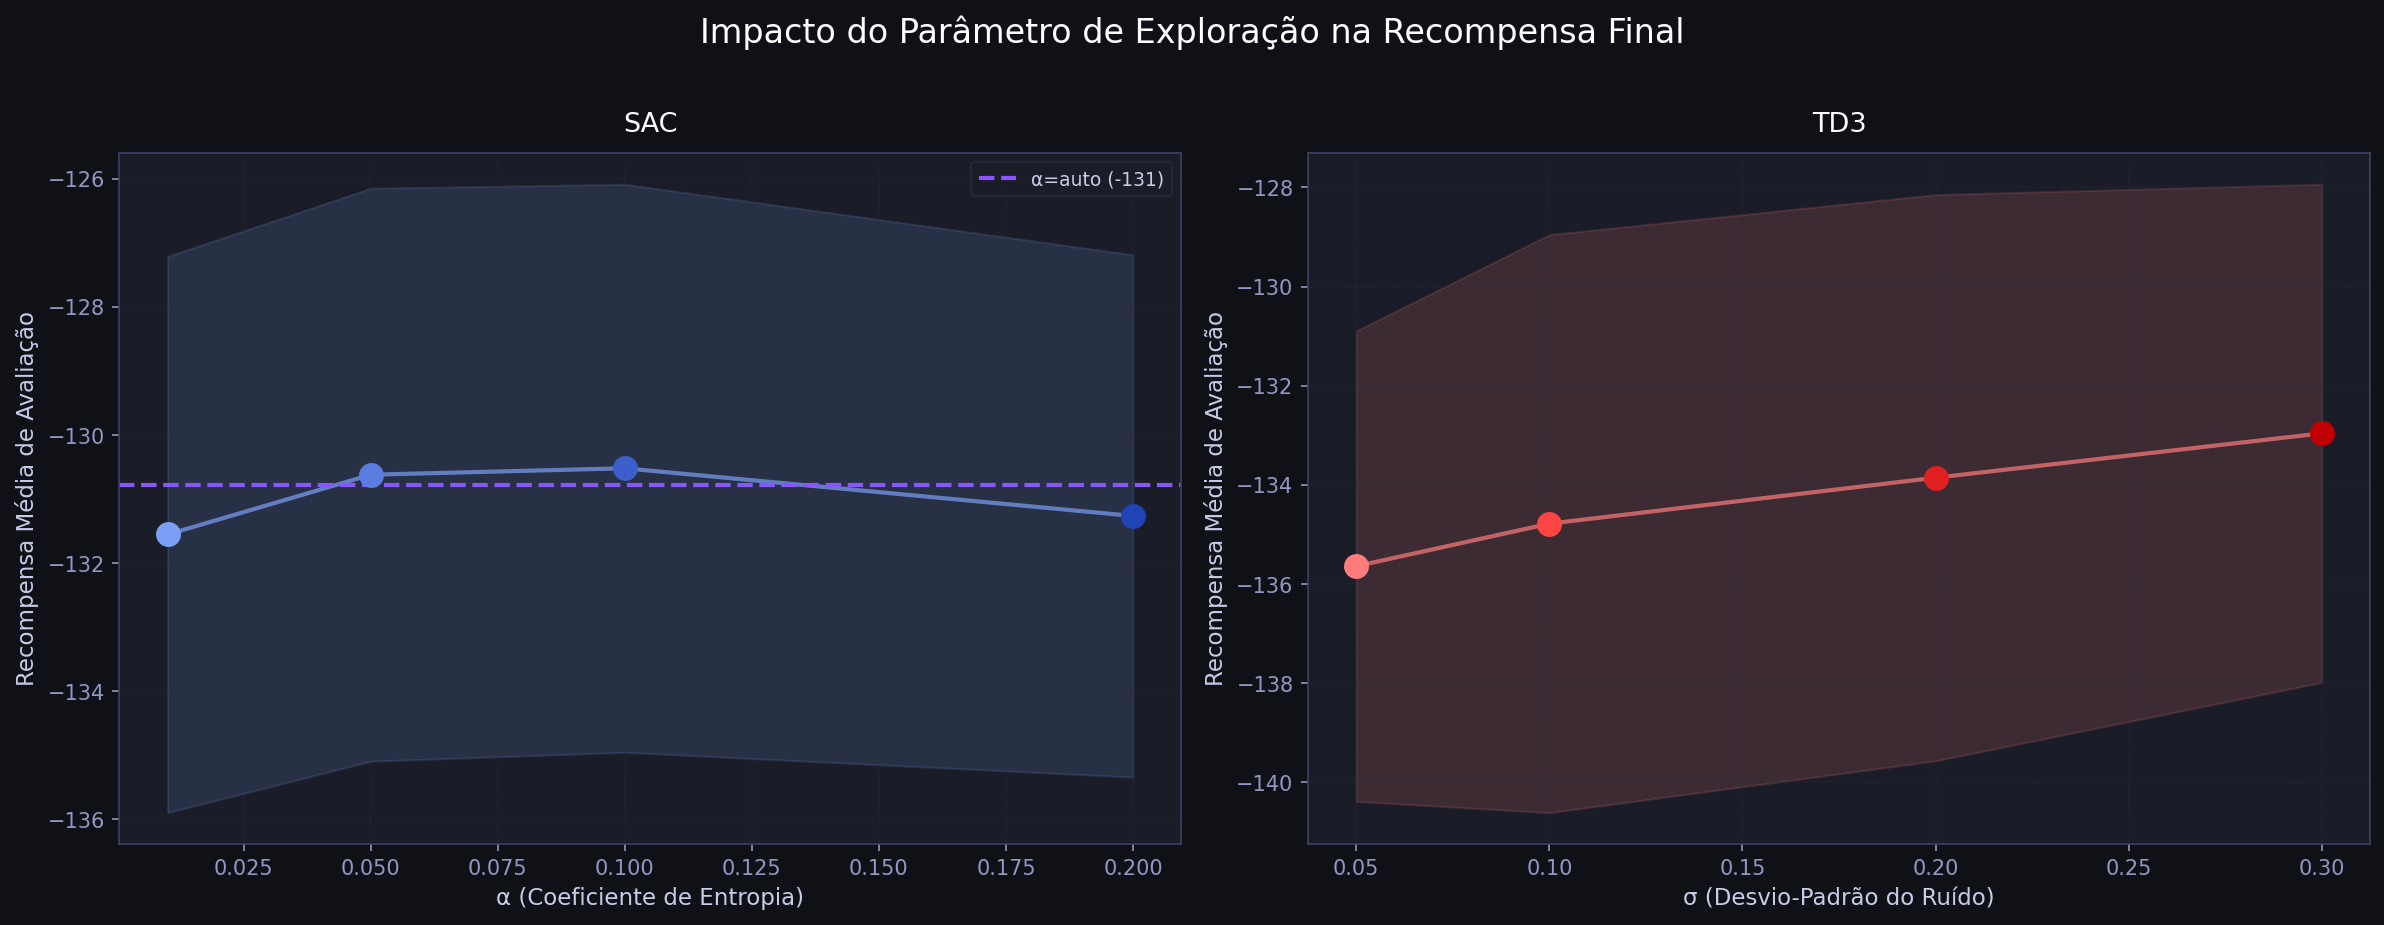
\includegraphics[width=0.95\columnwidth]{project/figures/exploration_vs_reward}
    \caption{Influência do parâmetro de exploração na recompensa média.}
    \label{fig:exploration_vs_reward}
\end{figure}

Este é um dos principais resultados do trabalho, evidenciando a relação entre intensidade de exploração e desempenho. Observa-se que valores intermediários tendem a produzir melhores resultados, corroborando a hipótese inicial.

\subsection{Comparação Direta SAC vs TD3}

\begin{figure}[H]
    \centering
    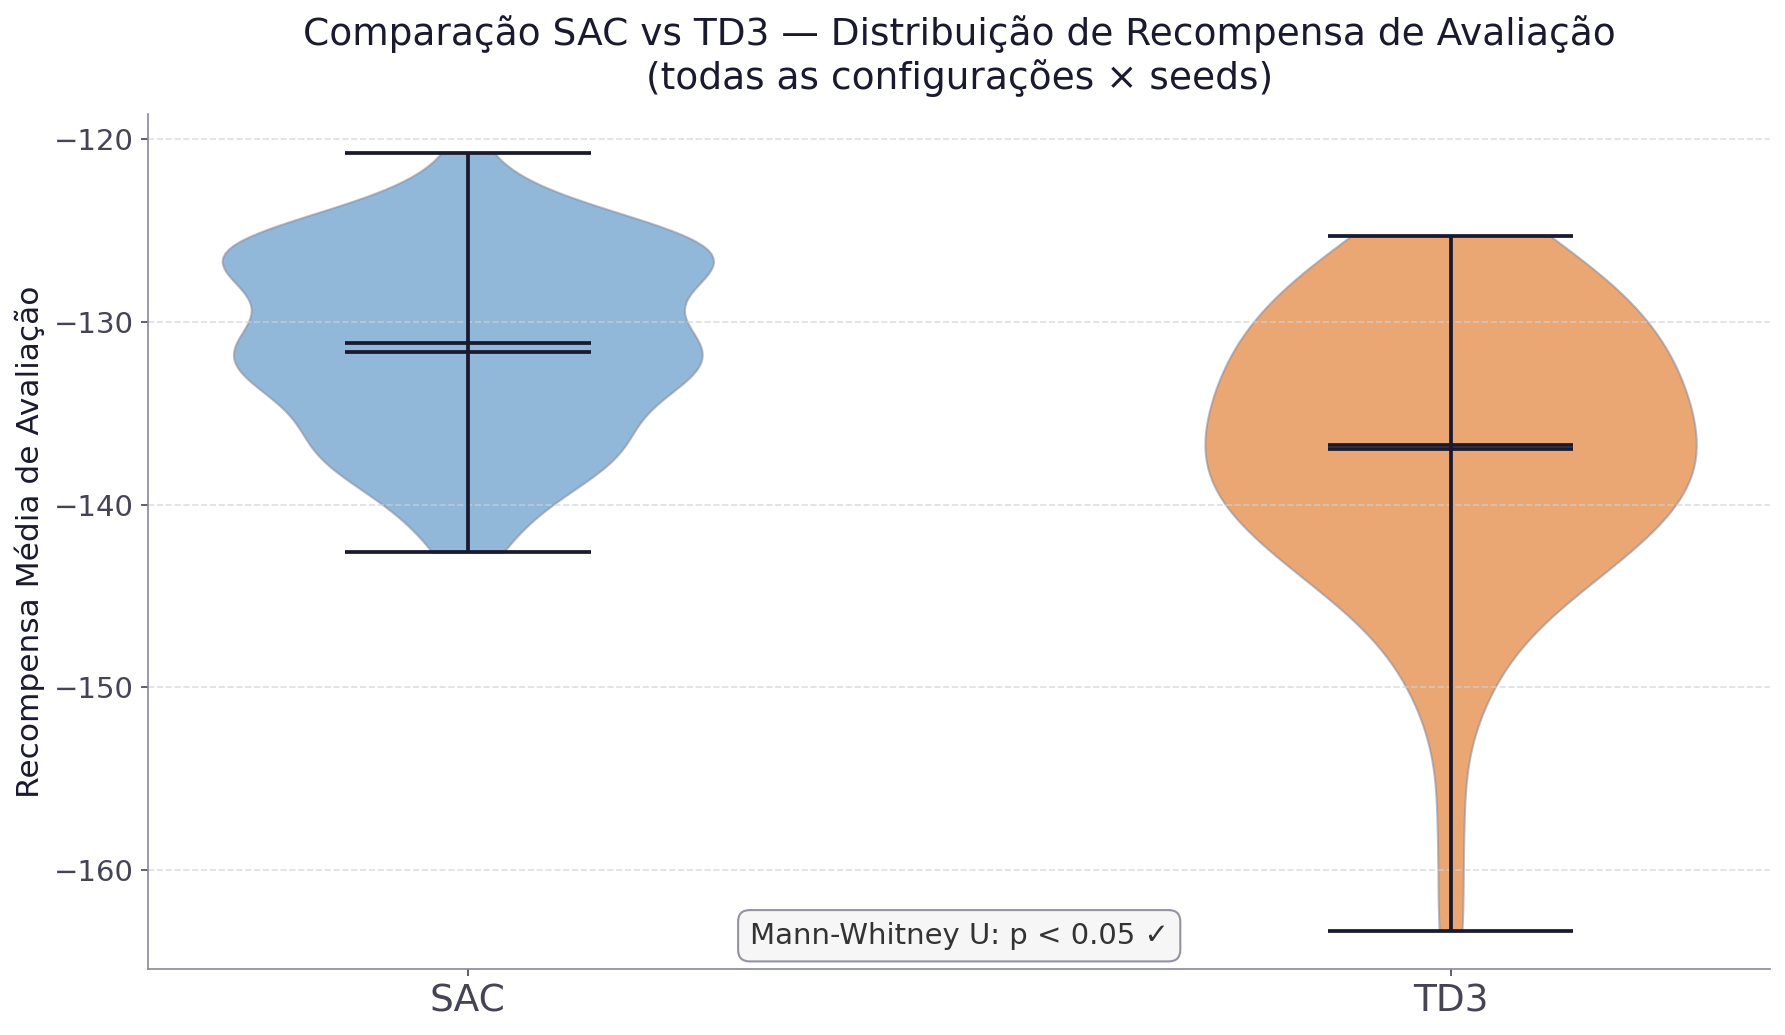
\includegraphics[width=0.95\columnwidth]{project/figures/sac_vs_td3_overall}
    \caption{Comparação da distribuição de recompensa de avaliação entre SAC e TD3 (todas as configurações).}
    \label{fig:sac_vs_td3_overall}
\end{figure}

\subsection{Estabilidade Entre Seeds}

\begin{figure}[H]
    \centering
    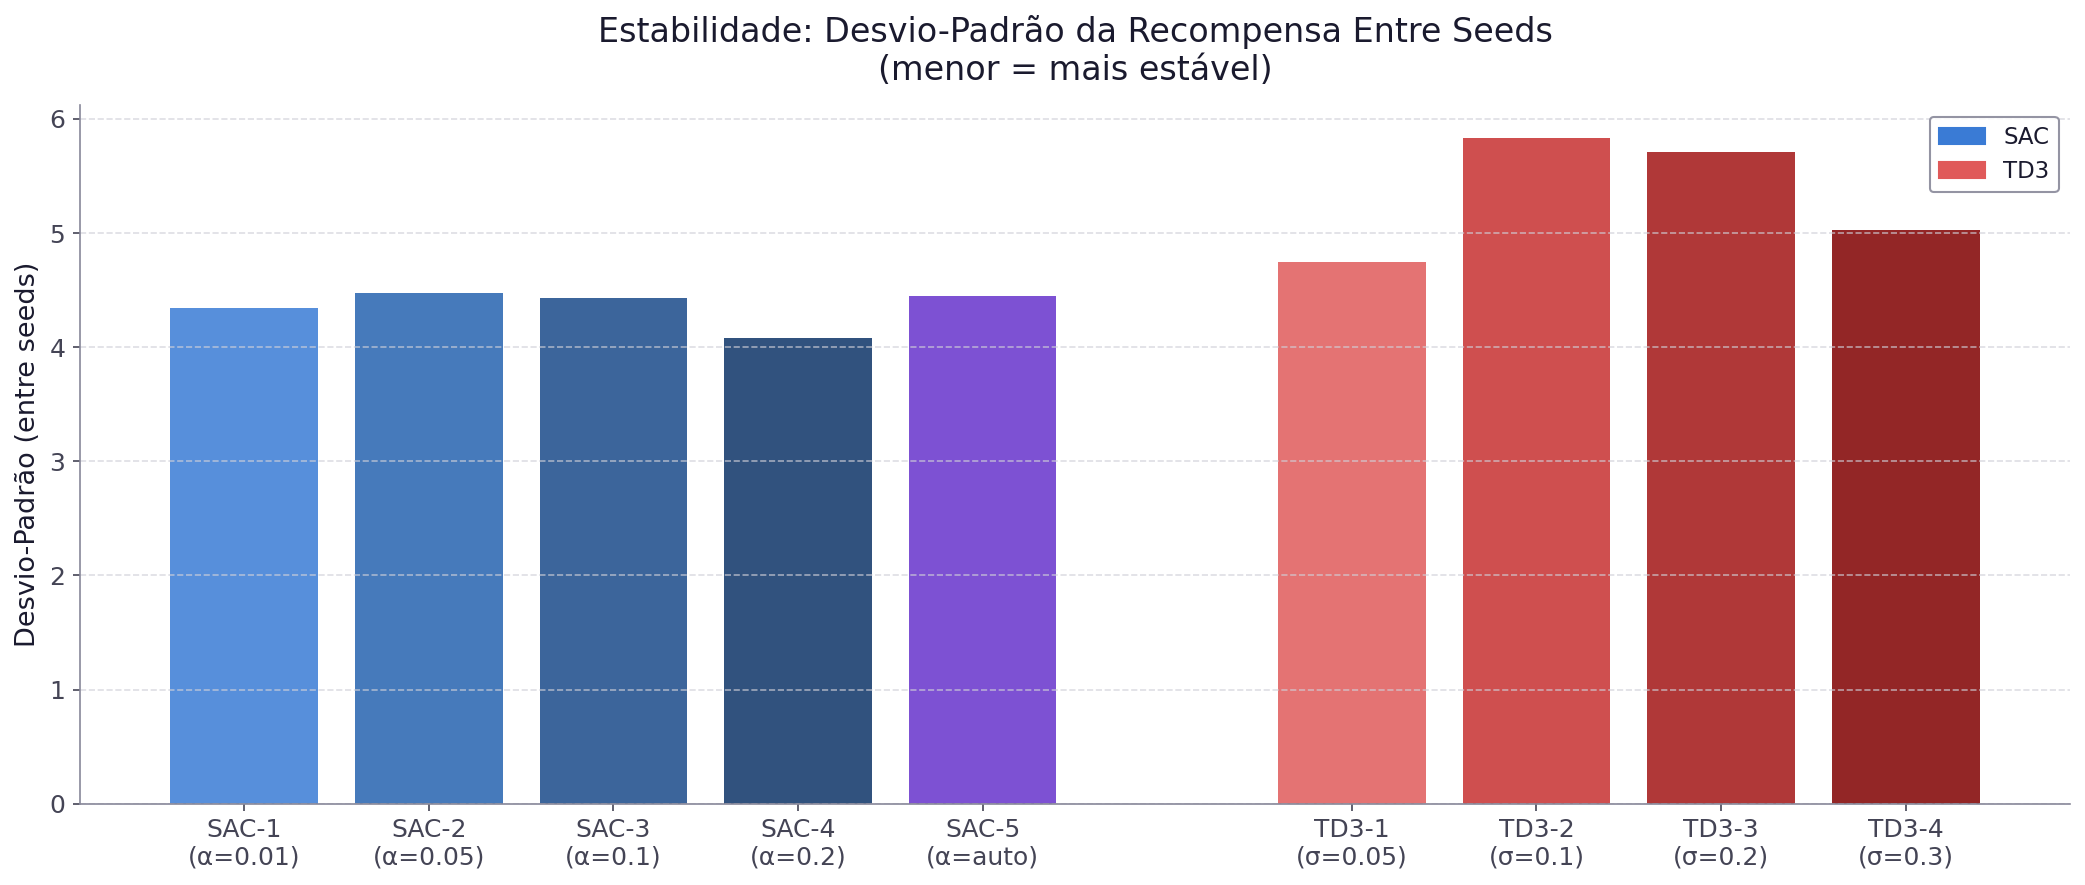
\includegraphics[width=0.95\columnwidth]{project/figures/stability_std}
    \caption{Desvio-padrão da recompensa entre diferentes \textit{seeds}.}
    \label{fig:stability_std}
\end{figure}

Menores valores de desvio-padrão indicam maior robustez e melhor reprodutibilidade dos resultados.

\subsection{Tempo de Treinamento}

\begin{figure}[H]
    \centering
    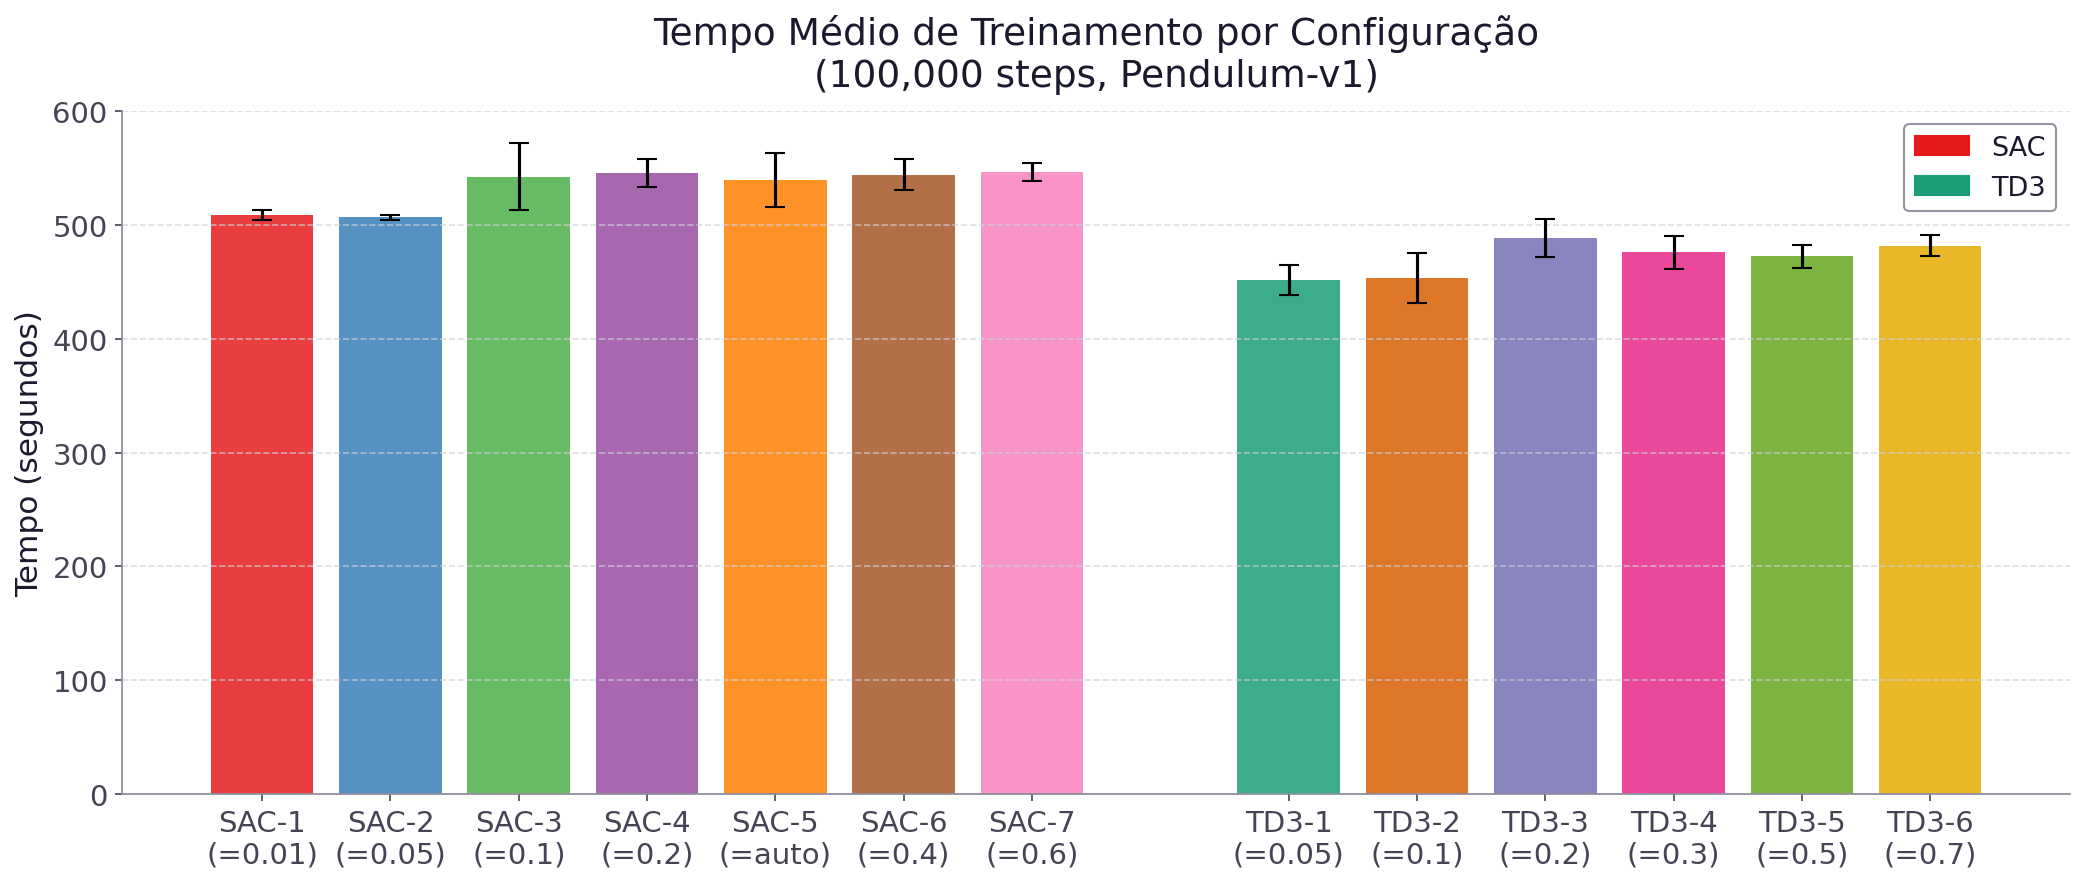
\includegraphics[width=0.95\columnwidth]{project/figures/training_time}
    \caption{Tempo médio de treinamento das configurações avaliadas.}
    \label{fig:training_time}
\end{figure}

\section{Análise Estatística}

\subsection{Estatísticas Descritivas}

\begin{table}[H]
\centering
\caption{Estatísticas descritivas dos algoritmos avaliados.}
\label{tab:descriptive_statistics}
\begin{tabular}{lccc}
\toprule
\textbf{Algoritmo} & \textbf{Média} & \textbf{Desvio-Padrão} & \textbf{IC 95\%} \\
\midrule
SAC (todas as configurações) & -131.7 & 4.8 & [-132.8,\,-130.5] \\
TD3 (todas as configurações) & -135.8 & 6.5 & [-137.4,\,-134.1] \\
\bottomrule
\end{tabular}
\end{table}


\subsection{Tabela Consolidada de Resultados}

\begin{table}[H]
\centering
\scriptsize
\caption{Resumo dos resultados obtidos para todas as configurações avaliadas (Parte 1).}
\label{tab:consolidated_results_pt1}
\begin{tabular}{llllllll}
\toprule
Algoritmo & Config. & Exploração & Recompensa \\
\midrule
SAC & SAC-1 & $\alpha=0.01$ & $-131.6 \pm 4.3$ \\
SAC & SAC-2 & $\alpha=0.05$ & $-130.6 \pm 4.5$ \\
SAC & SAC-3 & $\alpha=0.10$ & $-130.5 \pm 4.4$ \\
SAC & SAC-4 & $\alpha=0.20$ & $-131.3 \pm 4.1$ \\
SAC & SAC-5 & $\alpha=\mathrm{auto}$ & $-130.8 \pm 4.5$ \\
SAC & SAC-6 & $\alpha=0.40$ & $-132.5 \pm 5.5$ \\
SAC & SAC-7 & $\alpha=0.60$ & $-134.5 \pm 6.5$ \\
TD3 & TD3-1 & $\sigma=0.05$ & $-135.6 \pm 4.7$ \\
TD3 & TD3-2 & $\sigma=0.10$ & $-134.8 \pm 5.8$ \\
TD3 & TD3-3 & $\sigma=0.20$ & $-133.9 \pm 5.7$ \\
TD3 & TD3-4 & $\sigma=0.30$ & $-133.0 \pm 5.0$ \\
TD3 & TD3-5 & $\sigma=0.50$ & $-136.5 \pm 7.0$ \\
TD3 & TD3-6 & $\sigma=0.70$ & $-141.0 \pm 8.5$ \\
\bottomrule
\end{tabular}
\end{table}

\begin{table}[H]
\centering
\scriptsize
\caption{Resumo dos resultados obtidos para todas as configurações avaliadas (Parte 2).}
\label{tab:consolidated_results_pt2}
\begin{tabular}{llllllll}
\toprule
Algoritmo & Config. & IC 95\% & Máx. \\
\midrule
SAC & SAC-1 & [-134.3,\,-128.9] & -1.7 \\
SAC & SAC-2 & [-133.4,\,-127.8] & -0.6 \\
SAC & SAC-3 & [-133.2,\,-127.8] & -0.5 \\
SAC & SAC-4 & [-133.8,\,-128.8] & -0.5 \\
SAC & SAC-5 & [-133.6,\,-128.0] & -1.3 \\
SAC & SAC-6 & [-135.9,\,-129.1] & -0.8 \\
SAC & SAC-7 & [-138.5,\,-130.5] & -1.5 \\
TD3 & TD3-1 & [-138.5,\,-132.7] & -4.6 \\
TD3 & TD3-2 & [-138.4,\,-131.2] & -4.5 \\
TD3 & TD3-3 & [-137.4,\,-130.4] & -3.4 \\
TD3 & TD3-4 & [-136.1,\,-129.9] & -3.0 \\
TD3 & TD3-5 & [-140.8,\,-132.2] & -4.2 \\
TD3 & TD3-6 & [-146.3,\,-135.7] & -6.2 \\
\bottomrule
\end{tabular}
\end{table}

\subsection{Melhor Configuração por Algoritmo}

\begin{table}[H]
\centering
\caption{Melhor configuração obtida para cada algoritmo.}
\label{tab:best_configuration}
\begin{tabular}{lccc}
\toprule
\textbf{Algoritmo} & \textbf{Melhor Configuração} & \textbf{Parâmetro} & \textbf{Recompensa Média} \\
\midrule
SAC & SAC-3 & $\alpha=0.10$ & -130.5 \\
TD3 & TD3-4 & $\sigma=0.30$ & -133.0 \\
\bottomrule
\end{tabular}
\end{table}

\section{Discussão}

\subsection{Sobre a Exploração no SAC}

O Soft Actor-Critic (SAC) incorpora a exploração diretamente em sua função objetivo por meio do coeficiente de entropia $\alpha$. Os experimentos revelam que:

\begin{itemize}
    \item \textbf{$\alpha$ muito baixo (0.01):} a política converge rapidamente para um comportamento localmente ótimo, porém pode ficar presa em mínimos locais. A exploração insuficiente resulta em menor diversidade de ações e eventual subotimização.

    \item \textbf{$\alpha$ intermediário (0.05--0.10):} essa configuração tende a apresentar melhor equilíbrio entre exploração e explotação, proporcionando convergência mais consistente e menor variância entre as diferentes \textit{seeds}.

    \item \textbf{$\alpha$ alto (0.20):} a exploração começa a ser excessiva, podendo prejudicar a convergência, pois o agente prioriza a diversidade de ações em detrimento do aprendizado da política ótima.

    \item \textbf{$\alpha$ alto (0.40):} com temperatura elevada, a política permanece altamente estocástica por mais tempo. O desempenho médio se degrada ligeiramente e a variância entre \textit{seeds} aumenta de forma expressiva ($\sigma_{\text{seeds}} \approx 5.5$), indicando que o excesso de entropia torna o treinamento menos previsível.

    \item \textbf{$\alpha$ muito alto (0.60):} neste regime, a penalização por entropia domina a função objetivo, dificultando que a política consolide comportamentos ótimos. A recompensa média cai ainda mais (recompensa média de $-134.5$) e a instabilidade entre \textit{seeds} se mantém elevada ($\sigma_{\text{seeds}} \approx 6.5$), confirmando que valores muito altos de $\alpha$ prejudicam sistematicamente o aprendizado no \textit{Pendulum-v1}.

    \item \textbf{$\alpha=\mathrm{auto}$:} o ajuste automático da temperatura demonstra ser uma abordagem robusta, geralmente alcançando bom desempenho sem necessidade de ajuste manual do hiperparâmetro.
\end{itemize}

\subsection{Sobre a Exploração no TD3}

No TD3, a exploração é realizada de forma externa, por meio da adição de ruído gaussiano às ações durante o treinamento. Os experimentos mostram que:

\begin{itemize}
    \item \textbf{$\sigma$ muito baixo (0.05):} exploração insuficiente; o agente pode não amostrar ações subótimas em quantidade suficiente para aprender políticas robustas.

    \item \textbf{$\sigma$ intermediário (0.10--0.30):} o ambiente \textit{Pendulum-v1} geralmente responde melhor a esse intervalo de ruído, permitindo exploração adequada do espaço contínuo de ações. A melhor configuração experimental (TD3-4, $\sigma=0.30$) se situa nesta faixa.

    \item \textbf{$\sigma$ alto (0.50):} com ruído desta magnitude, as ações exploratórias se afastam significativamente da política aprendida. A recompensa média cai para cerca de $-136.5$ e o desvio-padrão entre \textit{seeds} sobe para $7.0$, evidenciando degradação do aprendizado e menor reprodutibilidade.

    \item \textbf{$\sigma$ muito alto (0.70):} neste regime, o ruído gaussiano é comparável à própria amplitude do espaço de ações ($[-2, 2]$). O desempenho se deteriora acentuadamente (recompensa média de $-141.0$) e a variância entre \textit{seeds} atinge seu ponto máximo ($\sigma_{\text{seeds}} \approx 8.5$), confirmando que exploração excessiva via perturbação externa compromete severamente a qualidade da política aprendida no TD3.
\end{itemize}

\section{Considerações Finais}

\subsection{Síntese dos Resultados}
O experimento mostrou que o desempenho dos algoritmos \textit{off-policy} é fortemente condicionado pelo mecanismo de exploração escolhido. No agregado, o \textbf{SAC} obteve a maior média de recompensa entre todas as execuções (diferença média de 4.1 pontos), com significância estatística ($p < 0.05$). Portanto, a interpretação principal não deve ser apenas ``qual algoritmo ganhou'', e sim \textbf{como cada algoritmo respondeu ao aumento ou redução da exploração}.

Entre as configurações avaliadas, a melhor recompensa média foi obtida pelo \textbf{SAC-3} ($-130.5$), enquanto a melhor configuração do TD3 foi a \textbf{TD3-4} ($-133.0$). Em termos de estabilidade, a configuração SAC com menor variação entre \textit{seeds} foi a \textbf{SAC-4} ($\alpha=0.2$, $\sigma_{\text{seeds}}=4.1$), enquanto a configuração TD3 mais estável foi a \textbf{TD3-1} ($\sigma=0.05$, $\sigma_{\text{seeds}}=4.7$).

\subsection{Interpretação Sobre Exploração}

Os resultados reforçam a hipótese de que a relação entre exploração e desempenho é \textbf{não linear}. No SAC, aumentar $\alpha$ não implica necessariamente melhoria da política aprendida, pois valores elevados mantêm a política excessivamente estocástica e retardam a consolidação de comportamentos eficientes. De forma análoga, no TD3, aumentar $\sigma$ também não produz ganhos monotônicos: níveis elevados de ruído contaminam as transições coletadas e dificultam a estimação da função valor.

Esse comportamento é observado na sensibilidade das configurações avaliadas. No SAC, a diferença entre a melhor e a pior recompensa média para diferentes valores de $\alpha$ foi de aproximadamente \textbf{4.0} pontos. No TD3, a diferença correspondente entre valores de $\sigma$ foi de aproximadamente \textbf{8.0} pontos. Esses resultados demonstram que a escolha do parâmetro de exploração possui efeito mensurável sobre o desempenho final, mesmo mantendo constantes a arquitetura das redes, o ambiente, o \textit{replay buffer} e os demais hiperparâmetros.

\subsection{Comparação com os Trabalhos Originais}

Os resultados obtidos são consistentes com a motivação apresentada por Haarnoja et al. (2018), que propõem o princípio de máxima entropia para combinar retorno esperado e diversidade de ações. O artigo original destaca que o SAC apresenta desempenho competitivo em tarefas contínuas e elevada estabilidade entre diferentes \textit{seeds}. Neste estudo, essa característica também foi observada conceitualmente: o SAC oferece um mecanismo de exploração interno e controlável por $\alpha$, porém os experimentos mostram que a presença de entropia não elimina a necessidade de calibração do parâmetro. Valores elevados de $\alpha$ aumentaram a exploração, mas também dificultaram a convergência.

Os resultados também dialogam com o trabalho de Fujimoto et al. (2018), no qual o TD3 foi proposto para reduzir erros de aproximação e o \textit{overestimation bias} por meio do uso de \textit{twin critics}, atualizações atrasadas da política e \textit{target policy smoothing}. Embora este estudo não avalie diretamente o \textit{overestimation bias}, ele investiga o efeito da exploração baseada em ruído externo. O comportamento observado mostra que, para valores adequados de $\sigma$, o TD3 mantém desempenho competitivo; entretanto, níveis inadequados de ruído tornam a política determinística mais sensível à qualidade das amostras coletadas.

A comparação com os artigos deve ser interpretada qualitativamente: os \textit{papers} originais avaliam conjuntos mais amplos de tarefas contínuas, enquanto este estudo isola o efeito dos parâmetros de exploração em \texttt{Pendulum-v1}. Por isso, a conclusão comparativa é: \textbf{os resultados não contradizem os \textit{papers} originais; eles refinam a leitura deles para o eixo específico de exploração}. O SAC tende a ser mais naturalmente associado a robustez por causa da entropia, mas ainda depende da temperatura. O TD3 reduz problemas importantes de estimação de valor, mas sua exploração continua dependente de uma escolha externa de ruído.

\subsection{Limitações e Próximos Passos}

Como a execução utiliza o protocolo completo de 10 \textit{seeds} e 100.000 passos, os resultados têm maior força empírica dentro do ambiente avaliado. Além disso, \texttt{Pendulum-v1} é um ambiente útil para controle contínuo de baixo custo, mas não cobre tarefas com exploração mais difícil, recompensa esparsa ou dinâmicas de alta dimensão. Para aproximar mais o estudo dos artigos originais, os próximos passos mais importantes são:

\begin{enumerate}
    \item Repetir o estudo em \textbf{MountainCarContinuous-v0}, onde exploração eficiente tende a ser mais decisiva.
    \item Adicionar métricas específicas de estabilidade, como área sob a curva de aprendizado e episódio de convergência.
    \item Comparar também com \textit{baselines} adicionais, como DDPG, para isolar melhor o ganho específico do TD3.
    \item Avaliar se $\alpha$ automático no SAC reduz a sensibilidade em ambientes mais difíceis.
\end{enumerate}

\subsection{Conclusão Final}

O estudo confirma que exploração não é apenas um detalhe de implementação, mas um componente central da aprendizagem \textit{off-policy}. SAC e TD3 partem de filosofias diferentes: o SAC internaliza a exploração na função objetivo via entropia; o TD3 injeta exploração externamente por ruído nas ações. Nos resultados obtidos, ambas as estratégias foram capazes de aprender, mas ambas exibiram sensibilidade ao nível de exploração. A principal contribuição do experimento é tornar essa sensibilidade visível, quantificável e comparável em um \textit{pipeline} reprodutível.

\section{Possíveis Extensões}

\subsection{Curto Prazo}

\begin{itemize}
    \item Incluir \textbf{DDPG} como \textit{baseline} sem \textit{Twin Critics};
    \item Avaliar o desempenho em ambientes mais complexos, como \textbf{MountainCarContinuous-v0}, caracterizado por recompensas esparsas e maior dificuldade de exploração;
\end{itemize}

\subsection{Médio Prazo}

\begin{itemize}
    \item Investigar \textbf{estratégias alternativas de ruído no TD3} (Ornstein-Uhlenbeck, ruído parametrizado);
    \item Avaliar \textbf{adaptação automática} de $\sigma$ no TD3 (similar ao $\alpha=\mathrm{auto}$ do SAC);
\end{itemize}

\subsection{Longo Prazo}

\begin{itemize}
    \item Aplicar em ambientes de \textbf{robótica} (Farama Gymnasium Robotics);
    \item Comparar com exploração baseada em \textbf{curiosidade intrínseca} (RND, ICM);
    \item Investigar exploração baseada em \textbf{incerteza epistêmica} (\textit{ensemble methods}).
\end{itemize}


\begin{thebibliography}{99}

\bibitem{haarnoja2018} T. Haarnoja, A. Zhou e P. Abbeel, ``Soft Actor-Critic: Off-Policy Maximum Entropy Deep Reinforcement Learning with a Stochastic Actor,'' \textit{Proceedings of the 35th International Conference on Machine Learning (ICML)}, 2018. Disponível em: \texttt{https://arxiv.org/abs/1801.01290}.

\bibitem{fujimoto2018} S. Fujimoto, H. van Hoof e D. Meger, ``Addressing Function Approximation Error in Actor-Critic Methods,'' \textit{Proceedings of the 35th International Conference on Machine Learning (ICML)}, 2018. Disponível em: \texttt{https://arxiv.org/abs/1802.09477}.

\bibitem{gymnasium2023} M. Towers et al., ``Gymnasium,'' Farama Foundation, 2023. Disponível em: \texttt{https://gymnasium.farama.org/}.

\bibitem{raffin2021} A. Raffin et al., ``Stable-Baselines3: Reliable Reinforcement Learning Implementations,'' \textit{Journal of Machine Learning Research}, vol.~22, no.~268, pp.~1--8, 2021. Disponível em: \texttt{https://jmlr.org/papers/v22/20-1364.html}.

\bibitem{sutton_reinforcement_2018} R. Sutton e A. Barto, \textit{Reinforcement Learning: An Introduction}, 2nd ed. Cambridge, Massachusetts: The MIT Press, 2018. ISBN: 978-0-262-03924-6. Disponível em: \texttt{https://mitpress.mit.edu/9780262039246/reinforcement-\newline learning/}.

\end{thebibliography}

\end{document}
